
\section{Robô}
robo etc.

\section{Molelo geométrico}

\begin{figure}[h]
	\centering
	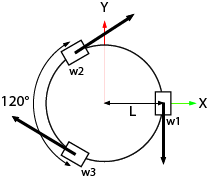
\includegraphics{figures/model}
	\caption{Modelo geometrico do robô de 3 rodas}
	\label{lof}
\end{figure}

\section{Matriz de translação}

\begin{gather}
	\begin{bmatrix} \dot{V}_{w1} \\  \dot{V}_{w2} \\  \dot{V}_{w3} \end{bmatrix}
	=
	\begin{bmatrix}
		0 & 2/3 & L/3 \\
		-1/\sqrt{3} & -1/3 & L/3\\
		1/\sqrt{3} & -1/3 & L/3
	\end{bmatrix}
	\cdot
	\begin{bmatrix} \dot{V}\cdot \cos{\theta} \\  \dot{V}\cdot \sin{\theta} \\  \dot{\omega} \end{bmatrix}
\end{gather}

\[ \overrightarrow{V} = (\dot{V}\cdot \cos{\theta} , \dot{V}\cdot \sin{\theta}) \]



\[\overrightarrow{V} \text{ :  Vetor velocidade linear do robô} \]  
\[\dot{V}_{w1}   \text{ :  Velocidade linear da roda 1} \]  
\[\dot{V}_{w2}   \text{ :  Velocidade linear da roda 2} \]  
\[\dot{V}_{w3}   \text{ :  Velocidade linear da roda 3} \] 
\[\dot{\omega}   \text{ :  Velocidade angular do robô a partir do centro de massa} \]  
\[L   \text{ :  Distância entre o centro de massa da roda e o centro de massa do robô} \]  



